%\vspace{-0.1in}
\section{Experiments and Results}
\label{s:results}

\xpkm{Sometimes authors describe all the treatments, then describe all the results.
Sometimes that works, but other times it is hard for the reader to keep everything straight.
For this paper, let's take the easier route, which is to introduce each treatment, then
give the results.  I find this "story-telling" approach is easier to follow.}

\xpkm{We need to decide if we are going to include any asymmetric results or not.  If so,
perhaps we can start with a subsection called "Asymmetric Sensor Placement." 
We also note that we let the number of sensors evolve, but did not observe convergence, 
so in the remaining results will fix the number of sensors at 6 and enforce symmetric placement.}

\begin{figure*}[!htb]
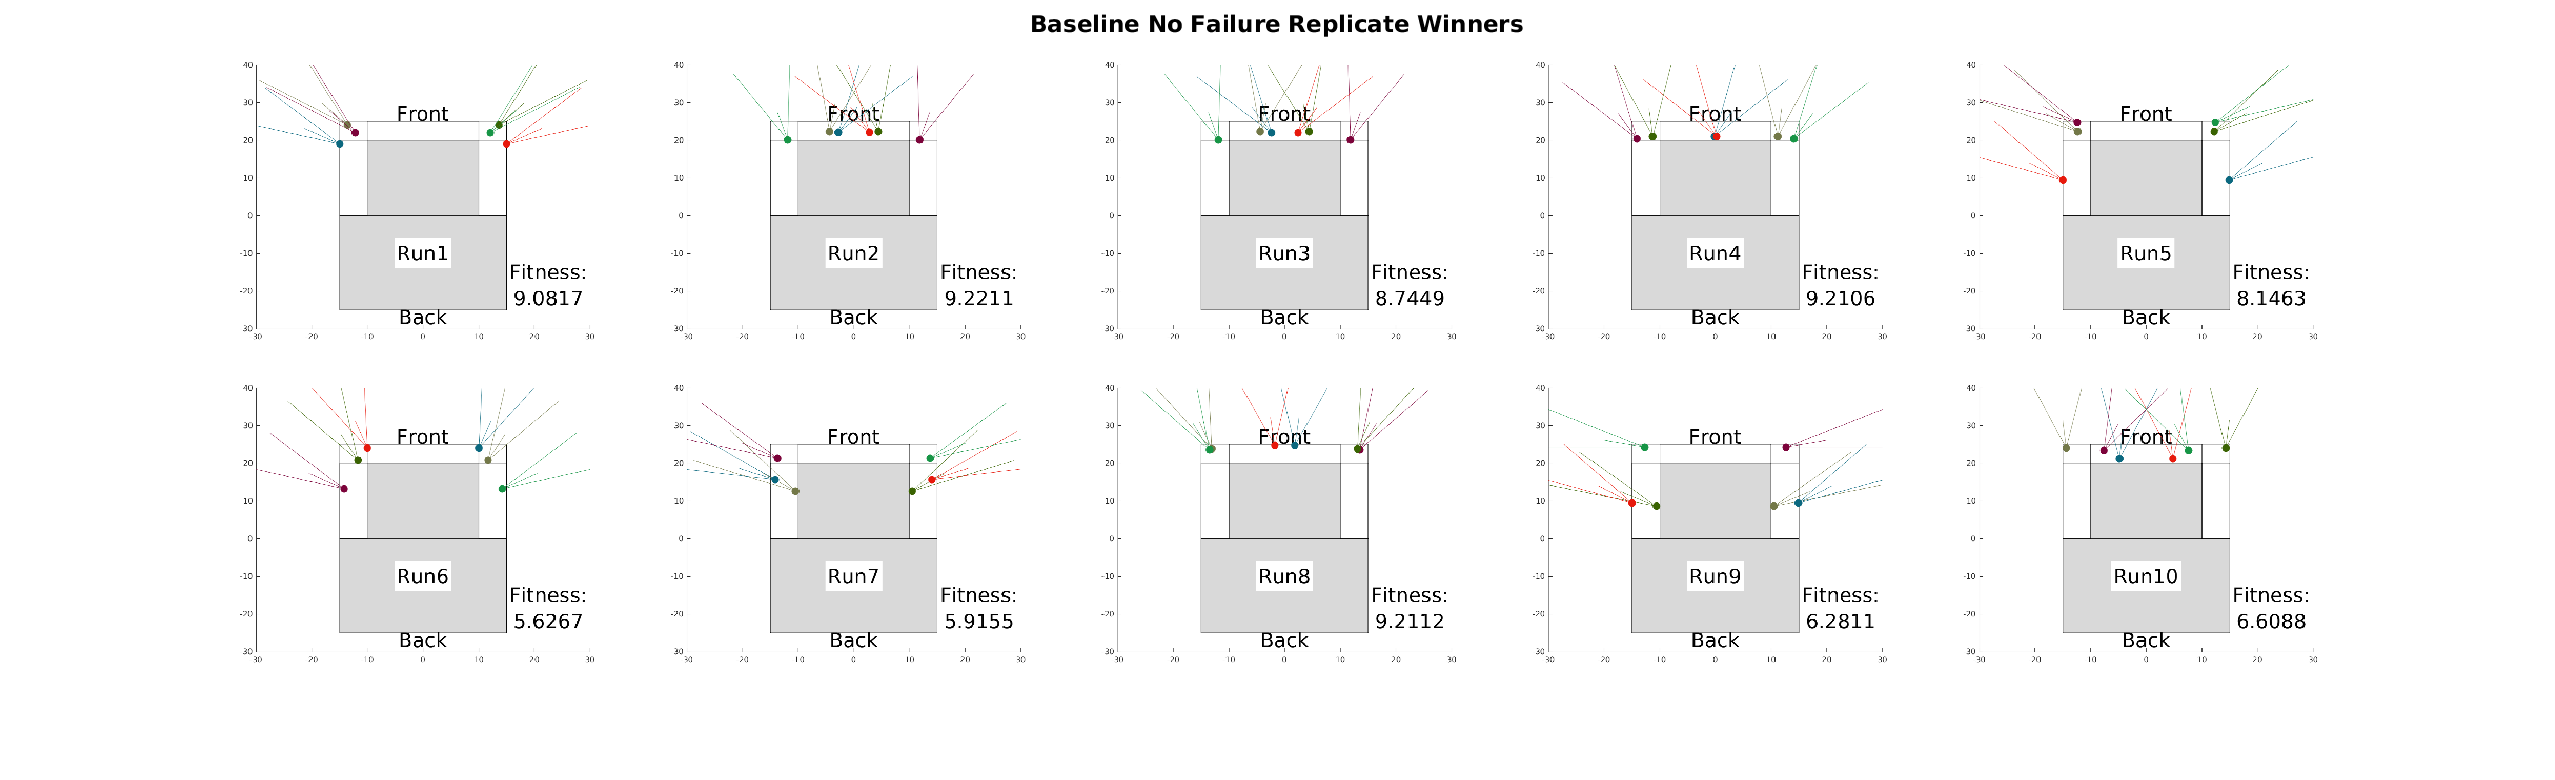
\includegraphics[width=1.0\textwidth]{Figures/6_sonar_symmetric_placement_without_failure_winners_panel_2x5.png}
     \vspace{-0.5in}
%      \includegraphics[width=0.9\textwidth]{Figures/6_sonar_symmetric_placement_without_failure_winners_panel_2X5-crop.pdf}
    \caption{A panel image showing the winning sensor configuration for each replicate in the baseline treatment experiment.}
    \label{baseline_panel_fig}
    \vspace{-0.05in}
\end{figure*}

As noted above, we present only a subset of the results of our experiments, where the
UGV was equipped with six sonar sensors, and left-right symmetry enforced.
We conducted three treatments.
%
First, a greenfield (idealized) scenario establishes a baseline of performance.  
%
%
In this treatment, no sensors fail during the mission and the vehicle
is able to operate under ideal conditions.  
In the next treatment, a single sensor randomly fails during the mission,
simulating a situation where an electrical or mechanical failure arises in the robot.  
%
The final treatment simulates physical damage to the vehicle,
wherein multiple sensors can fail based on their physical proximity to each other.  
We next describe the details of the evolutionary runs, followed by results for each treatment.

%Three different variations of experiments were conducted to evaluate the optimal sensor configuration for six sonar sensors; a greenfield scenario where no sensors fail during the mission, an emulated electrical or mechanical failure scenario where one sensor stops reporting any data partial through the mission mimicking events such as water damage or a broken connection to the sensor, and an impact related failure scenario simulating the rover making a hard collision with an object and incapacitating multiple sensors based on their spatial correlation. 


%%%%%%%%%%%%%%%%%%%%%%%%%
%\vspace{-0.1in}
\paragraph{Evolutionary Parameters}
Table~\ref{GA_param_table} lists the parameters of
the GA used in this study.
%
%
Each individual of the population represents a viable sensor configuration.
% , with the individual's chromosomes containing encodings of multiple sensor locations, relative to the center of the 
% UGV, and orientations.
Specifically, the genome of an individual consists of six behavioral traits relating to six individual sonar sensors. Each of these traits contain four values: a string describing the type of sensor such as 'sonar', the $x$ and $y$ position values of the sensor on the rover as well as a $z$ value that determines the angle at which this sensor should face.
%
After the  population has been evaluated in the simulation environment, tournament selection, with a tournament size of two, creates a parent pool. 
%
Members of the parent pool produce the children pool using crossover with a probability of $0.25$.
%
If crossover does not occur, a child is cloned from a parent.  
%
The original population and the new individuals present in the children pool are combined into the candidate pool, which is larger than the original population size. 
%
A fraction of the members of the candidate pool will randomly undergo mutation,
where the location and/or orientation of one or more sensors can be changed.
%
If mutation or crossover create a new individual, it is marked as unevaluated.  
%
All such individuals are then evaluated via Evo-ROS
before the next generation's population is selected.
%
Elitism is used to maintain the highest performing individual with the rest of the population filled by performing tournament selection.
%%%%%%%%%%%%%%%%%%%%%%%%%
\vspace{-0.1in}
\begin{table}[h!]
    \caption{Genetic Algorithm Parameters.}
    \vspace{-0.15in}
	\centering
    \begin{tabular}{|| c | c ||}
    	\hline
        Population Size & 30 \\
        Generations & 25 \\
        Mutation Probability & 0.15 \\
        Crossover Probability & 0.25 \\
        \hline
    \end{tabular}
    \label{GA_param_table}
%   \vspace{-0.1in}
\end{table}
%%%%%%%%%%%%%%%%%%%%%%%%%

% \begin{figure}[ht]
% 	\centering
%     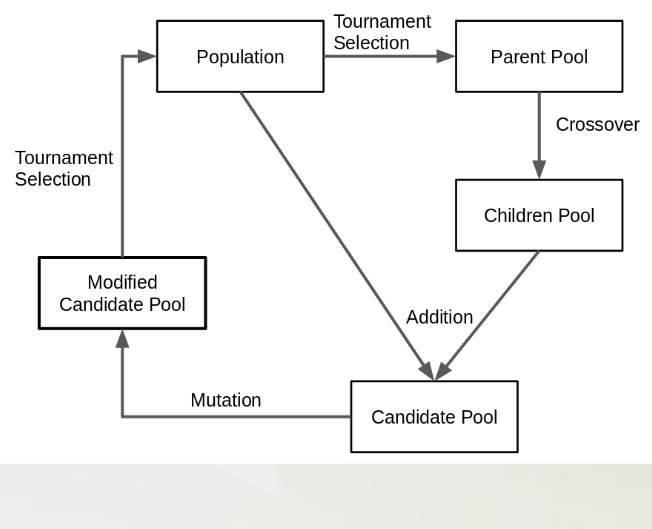
\includegraphics[width=0.4\textwidth, trim={0 1.9cm 0 0}, 		clip]{Figures/GAfigure.PNG}
%     \caption{Model of the GA.}
%     \label{ga_model_fig}
% \end{figure}



% \jmm{TODO: We should move the sensor constraints~(physical location, orientation, symmetry, up to the platform section.

% We are modeling our simulated system after a real rover with hardware already placed on the rover so we must limit the areas in which sonars are placed to the outer 5cm on the front half of the rover. The navigation controller being used never attempts to drive in reverse, so we do not consider the placement of any sensors on the rear half of the rover. The valid areas of sensor placement on the rover are shown in figure \ref{ga_search_space_fig}. We also included some constraints on the orient of the sensor based on the positional coordinates. This pre-engineering does not allow the sensor orients to be faced toward the rear of rover. For this study, the number of sensors is fixed at six and the configurations are required to be symmetric about the y-axis of the rover (left / right symmetry).
% }


% \begin{figure}[ht]
% 	\centering
%     \includegraphics[width=0.4\textwidth]{Figures/rover_sensor_placement_space.PNG}
%     \caption{Sensors can be placed on the outer 5cm on the front half of the robot.}
%     \label{ga_search_space_fig}
% \end{figure}

%Sensor configurations in each experiment were evaluated by equipping them on a simulated rover and allowing the rover to attempt to carry out the mission described in section \ref{s:rover} in three different environments.
% While the mission in each environment remained the same, both the type and the distribution of obstacles that the rover encountered were changed drastically. Between the three environments, the rover was exposed to tall walls, one meter wide cubes, and short cider blocks that had a height just below the height of sensors on the rover. The cider blocks height is important because it makes them insensible at close distances since they are too close to the ground, but visible at distances greater than about half a meter due to the nature of a sonar's conic sensing detecting a wider area the further the distance from the rover. We believe that this invisibility of objects at close distances to the rover will force the rover to choose better paths through clusters of objects, giving a soft distance between each obstacle that it passes rather than approaching it as close as possible without hitting it.  
%  detecting a wider area the further the distance from the rover.  We believe that this invisibility of objects at close distances to the rover will force the rover to choose better paths through clusters of objects, giving a soft distance between each obstacle that it passes rather than approaching it as close as possible without hitting it.

A controller/sensor configuration is evaluated by measuring
the performance of the UGV on waypoint following and obstacle avoidance tasks in 
three different environments, discussed in Section~\ref{s:rover}.   
%
Obstacles in the environments include tall walls, one meter wide cubes, and cinder blocks that are shorter than the height of sensors on the rover. 
%
Cinder blocks thus pose a potential challenge as they are
visible to the rover only at distances greater than 0.5 meters,
due to the cone shaped detection area of a sonar.
%  detecting a wider area the further the distance from the
% rover.
%
We suspect that the cinder blocks will force the vehicle
to evolve navigation strategies
that maintain a distance threshold from obstacles in order
to avoid losing the ability to detect very close objects.

Ten replicates are conducted per experiment. 
%
While this number is considered low for ER experiments, 
the simulation of each mission is computationally expensive 
and is limited to real time due to the use of Ardupilot. 
%
%Ardupilot is built around an inherent 400Hz loop, which limits 
%speed of the Gazebo simulator. 
%
An individual replicate takes between 16 and 24 hours of wall clock time, depending on the average performance of individuals in the replicate.
Attempting to run simulations faster than real-time results in random behavior,
as we cannot assure the control signals are consistent across multiple simulations
of the same controller/sensor configuration. 
%
We plan to address this in future work by replacing the Ardupilot control stack
with a custom autopilot stack, enabling faster than real time simulation. 
%
That said, a goal of this initial case study was to apply evolution to a target system
{\em exactly} matching one from the robotics community, including the use of Ardupilot.


\xpkm{Describe other features of the setup, including the waypoint tasks, fitness calculations, etc.
(note: if we do not include asymmetric runs, the features common to ALL runs can be discussed 
in the introductory material of this section).  
In the following subsections, we will note that the 
treatment is the same as the baseline, except for X, Y, Z.}

%In the baseline treatment, the rover is equipped with six sensors and symmetry is enforced and all sensors work ideally, always reporting on time with accurate data, during the evaluation. This explores the baseline optimal configuration of sensors for a rover. Ten replicates of this baseline treatment were commuted and the winning configurations from each run can be seen in figure \ref{baseline_panel_fig}. An overlay of all of the sensor placements and viewing areas can be seen in figure \ref{baseline_overlay_fig}.

%It can be seen in figure \ref{baseline_panel_fig} that two main patterns appear from this experiment. First, one that is more traditionally accept being an array of sensors placed across the front of the rover with slightly varying angles. This configuration gives the rover a full coverage of the environment directly in front of itself as well as sightly to its sides. The other configuration that emerges is having all of the sensors focus on coverage to the sides of the rover. Well neglecting viewing directly in front of the rover may seem like a weakness, we believe that these configurations are able to thrive because of an artifact of the Ardupilot waypoint navigation behavior. Ardupilot native behavior commonly has the rover drive in a serpentine pattern towards waypoint, causing the front of the rover to swing in an arc up to 60 degrees in magnitude. The driving patterns results in sensors that are mounted facing the side of the rover to detect that are directly in line between the rover's current position and its next waypoint as well as providing extra information to the controller about the environment to the sides of the rover.

%\vspace{-0.1in}
\paragraph{Baseline Experiments}
The UGV is equipped with six sensors and symmetry is enforced across experiments.  
%
In the first treatment, all sensors perform nominally, reporting on time with accurate data.  
%
Figure~\ref{baseline_panel_fig} shows the sensor configuration of best performing
individual in each replicate.  
%
Two main configurations emerge.
%
First is an array of sensors spread across the front of the vehicle,
with slightly varying angles. 
%
This configuration gives the UGV full sonar coverage directly in front, and sightly to its sides. 
%
Second, the sensors ``drift'' toward the sides of the vehicle.
%
Neglecting frontal coverage may seem like a weakness, but it appears that this configuration exploits an artifact of Ardupilot's waypoint navigation behavior. 
%
Specifically, the UGV drives in a serpentine pattern towards each waypoint, causing the orientation of the rover to swing in an arc of up to 60 degrees. 
%
Sensors mounted facing the side of the rover thus sweep through the area in front of the rover, while also providing information to the controller about the peripheral environment.



Figure~\ref{baseline_overlay_fig} overlays the results of the 10 replicates
on a single rover.
%
Common sensing cones and placement are indicated by darker shaded areas.  
%
As seen in Figure~\ref{baseline_panel_fig}, the sensors primarily sweep the forward viewing cone or cover the sides.

\begin{figure}[ht]
	\centering
    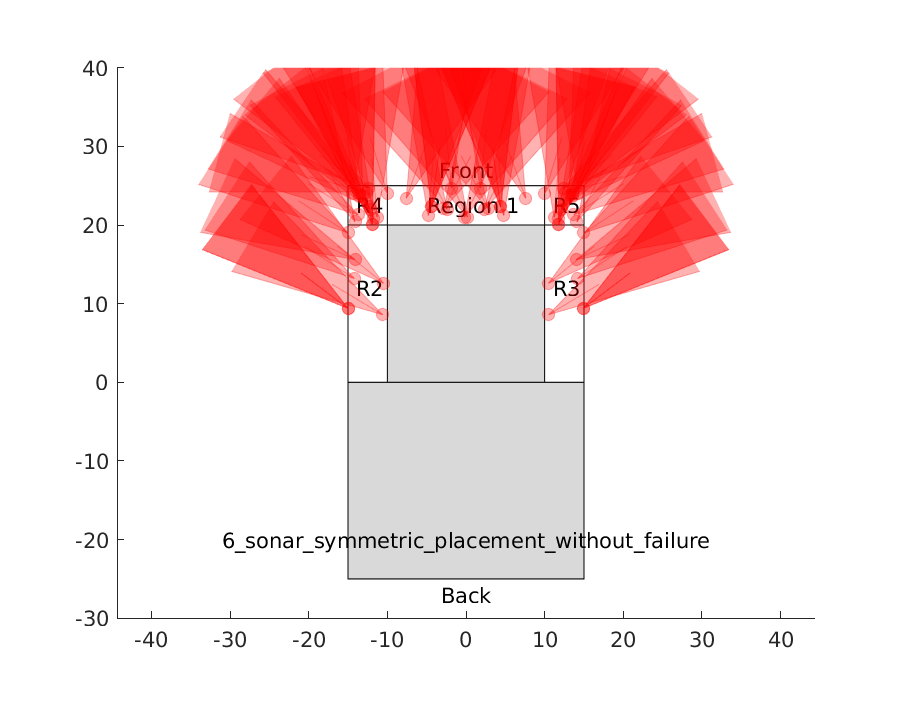
\includegraphics[width=0.5\textwidth]{Figures/6_sonar_symmetric_placement_without_failure_sensor_viewing_area_overlay.png}
    \vspace{-0.45in}
    \caption{Overlay of sensor placements and viewing areas from 10 replicates of the baseline treatment experiment.}
    \label{baseline_overlay_fig}
%    \vspace{-0.1in}
\end{figure}


\xpkm{Need to add a paragraph describing Figure~\ref{evol_track_fig}.
Include or compare with any other plots of evolutionary trajectory?}
A scatter plot of the evolutionary progress of a sample run is shown in Figure~\ref{evol_track_fig}. Here each individual is plotted according to its fitness score and generation. Individuals are color-coded based on their generation, thus individuals from the same generation share the same color. The fitness of the best fit individual and the average fitness for the generation are also plotted. It can be seen that most increases in fitness take place during the first 15 generations, after which fitness plateaus, and the average fitness for each generation approaches that of the most fit individual.
\xjmm{Figure~\ref{evol_track_fig} is currently problematic.  The legend is ambiguous.  It should clearly show best and average, which I assume are the lines on the plot, not the circles.  Perhaps make the best a solid line and the average a dashed line.}

\begin{figure}[ht]
%	\vspace{-0.15in}
	\centering
    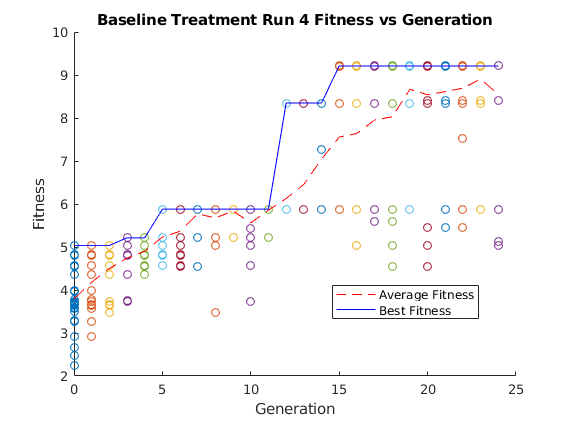
\includegraphics[width=0.45\textwidth]{Figures/fitness_vs_generation_editted.png}
    \caption{Plots of the average and best fitnesses in the population over 25 generations for a sample replicate of the baseline treatment.}
    \label{evol_track_fig}
    \vspace{-0.1in}
\end{figure}

\xpkm{Note treatment same as above but with random failures.
Include specific details of the failure model(s).
Then go on to present results.}

%In the random sensor failure experiment, one random sensor will stop reporting any data at a randomly selected point of time between 40 and 80 seconds into the mission. To put this time into perspective, the rover is allowed 540 seconds to complete the mission with the optimal time being between 360 and 400 seconds depending on the distribution of obstacles in the environment. This means that the failure of a sensor is likely to occur at some point between the first and second waypoint during the first leg of the mission. 

% \vspace{-0.1in}
\paragraph{Random Sensor Failures}
In the second treatment, a randomly
selected sensor fails between 40 and 80 seconds into an individual simulation.
%
The UGV is allowed 540 seconds to complete a mission,
with the optimal time being between 360 and 400 seconds,
depending on the distribution of obstacles. 
%
% Failure of a sensor occurs at some point between the first and second waypoint during the first leg of the simulation. 
%

% JMM: I think this is redundant.  Mentioning that the sensor fails should be sufficient for this community.
%Failures on this platform are simulated by passing the raw Gazebo sensor feeds through a Sonar Filter process managed by Evo-ROS as can be seen in figure \ref{evo_ros_digram}. The Sonar Filter is a lightweight process that typically just relays the raw sensor data to the ROS based navigation controller, however to simulate failing sensors the data for each sensor can be manipulated before being relayed or not relayed at all. In the case of the random failure experiment, at the start of the simulation the Sonar Filter selects a random sensor which will fail and a time between 40 and 80 seconds for when the failure will occur. Once the selected time is reached, the Sonar Filter stops relaying any data from the ``failed'' sensor for the rest of the simulation. From that point on navigation control only has access to 5 out of the 6 sensors on the rover.

\xgas{Just added the following paragraph about random failure results. Please feel free to edit.}

% Figure \ref{random_failure_panel_fig} shows the best performing 
% individual for each of the ten replicates. 
Sensor placement for the random failure treatment was similar to the baseline treatment.  
%
Again two configurations emerge, the array of sensors across the front of the vehicle and
also spread along both sides. 
%
However, the results of this treatment evolve configurations with redundant sensors
 placed next to each other. 
%
In six of the ten replicates, redundancy is built into the configuration by having two sensors with nearly identical placement and orientation. 
%
Even when two sensors are not nearly identical in placement, evolved solutions tend to have multiple sensors dedicated to covering the same area.  
%
It appears that,  in the case of random failures, evolution favors redundancy over a wider sensing capability.

% \begin{figure*}[!htb]
% 	\centering
%     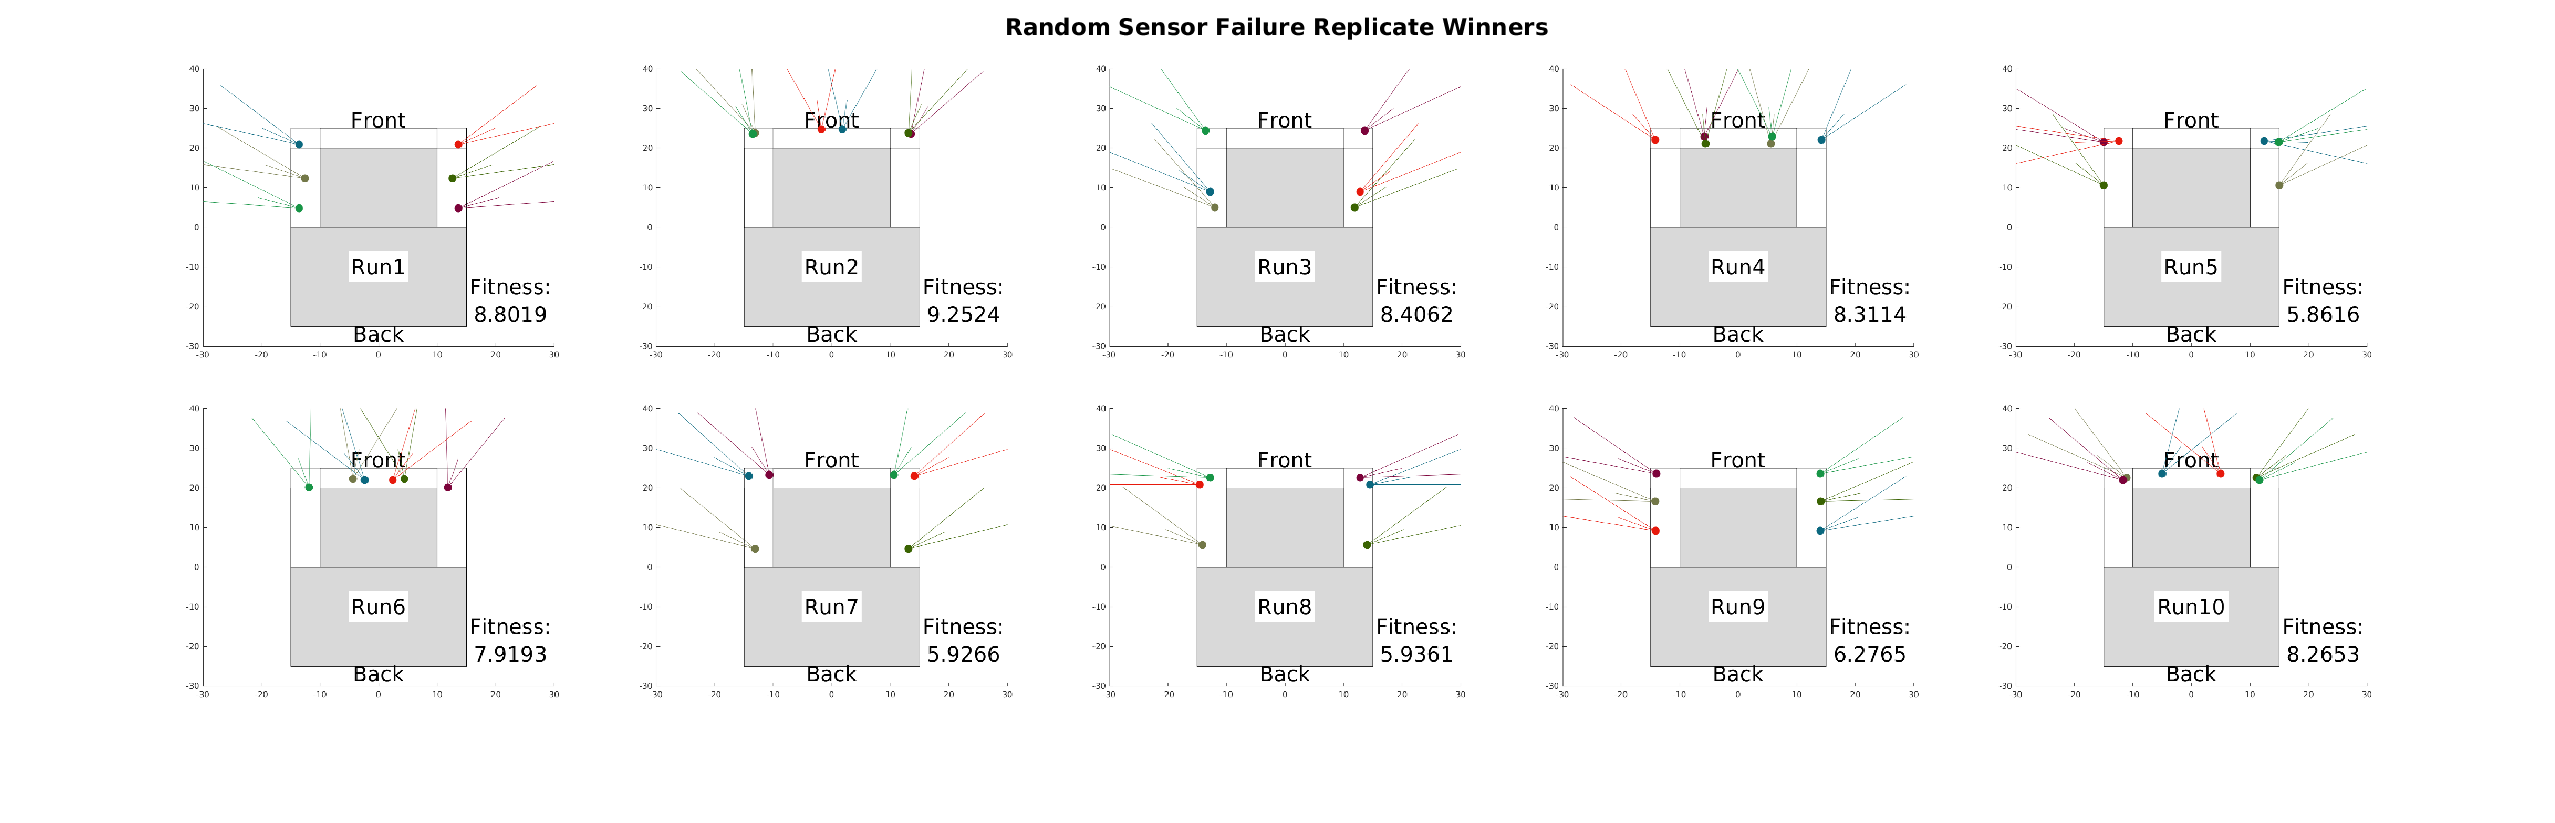
\includegraphics[width=0.95\textwidth]{Figures/6_sonar_symmetric_placement_with_complete_failure_winners_panel_2X5}
%     \caption{A panel image showing the winning sensor configuration for each replicate in the Random Failure Treatment.}
%     \label{random_failure_panel_fig}
% \end{figure*}

% \vspace{-0.1in}
\paragraph{Spatially Correlated Sensor Failure}

%This treatment explores the placement of sensors in situations where 
%sensor failures are correlated spatially, for example, due to physical
%damage in to an area of the vehicle.
%The configuration is is the same as in the previous treatment, with the 
%exception of the sensor failure model.
%In this treatment, at the start of each simulation a random time for failure is selected between 40 and 80 seconds, as was the case with the random failure scenario. However, now at the time of failure a random sensor is selected by the Sonar Filter process. This sensor is the considered to be the point of impact for the damage. From this sensor, three concentric circles are formed with radii of 3, 6, and 9cm, shown in figure \ref{spatial_failure_model}. Sensors within 3cm of the point of impact are guaranteed to fail. Sensors within 6 and 9cm have a 75 and 50\% chance of failing respectively. The Sonar Filter does not relay any data from a failed sensor and failed sensors do not have the chance to become active again for the duration of the mission.

Spatially correlated sensor failure simulates physical damage to a robot.  
%
Figure~\ref{spatial_failure_model} depicts
the spatial failure model centered on a sensor selected at random.  
%
Sensors within the affected area are also damaged and stop reporting.  
%
We hypothesize that this will pressure the sensors to be more evenly distributed across the robot and perhaps also demonstrate redundancy of coverage among the six sensors.  



\begin{figure}[ht]
%	\vspace{-0.1in}
	\centering
    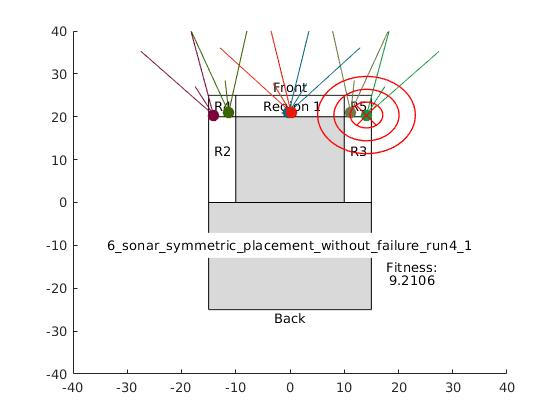
\includegraphics[width=0.4\textwidth]{Figures/6_sonar_failure_model.jpg}
    \vspace{-0.15in}
    \caption{The areas impacted by the spatially correlated failure model on a sample sensor configuration.}
    \label{spatial_failure_model}
%    \vspace{-0.15in}
\end{figure}

Figure~\ref{spatial_failure_panel_fig} plots the sensor placement of the highest performing individual in each of the ten replicates.
%
As in the baseline treatment, two primary configurations evolve.
%
The first remains an even spread of sensors across the front face of the rover.  
%
The second is focused on the sides of the platform.  
%
Surprisingly, there are clusters of sensors that would fall within the failure radius of the model.  
%
Apparently, the position of these sensors is more important than the risk of damage from sensor failures.    

% \begin{figure}[ht]
% 	\centering
%     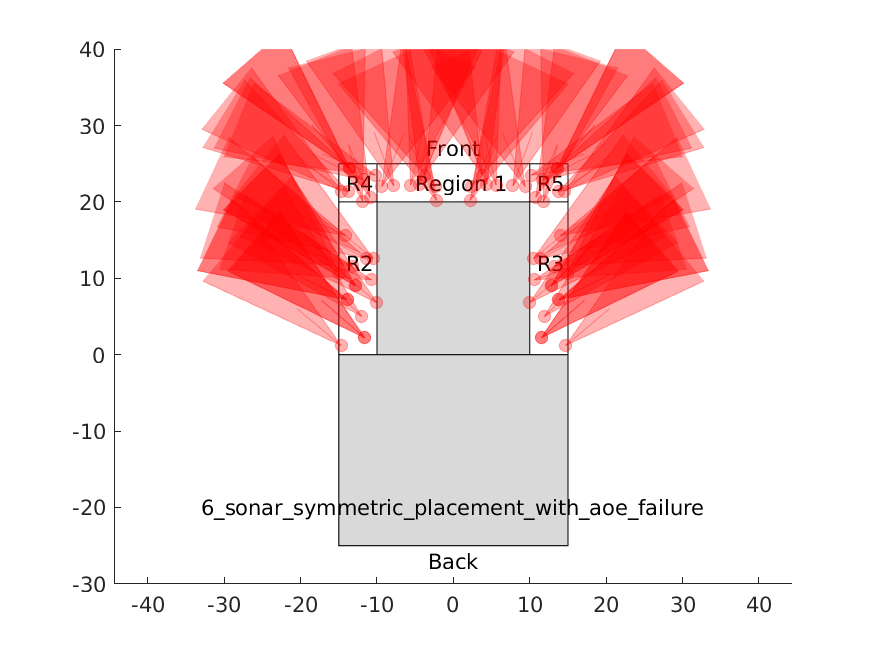
\includegraphics[width=0.4\textwidth]{Figures/6_sonar_symmetric_placement_with_aoe_failure_sensor_viewing_area_overlay.png}
%     \caption{Overlay of sensor placements and viewing areas from 10 replicates of the spatially correlated failure treatment experiment.}
%     \label{spatial_failure_overlay_fig}
% \end{figure}


\begin{figure*}[!htb]
	\centering
    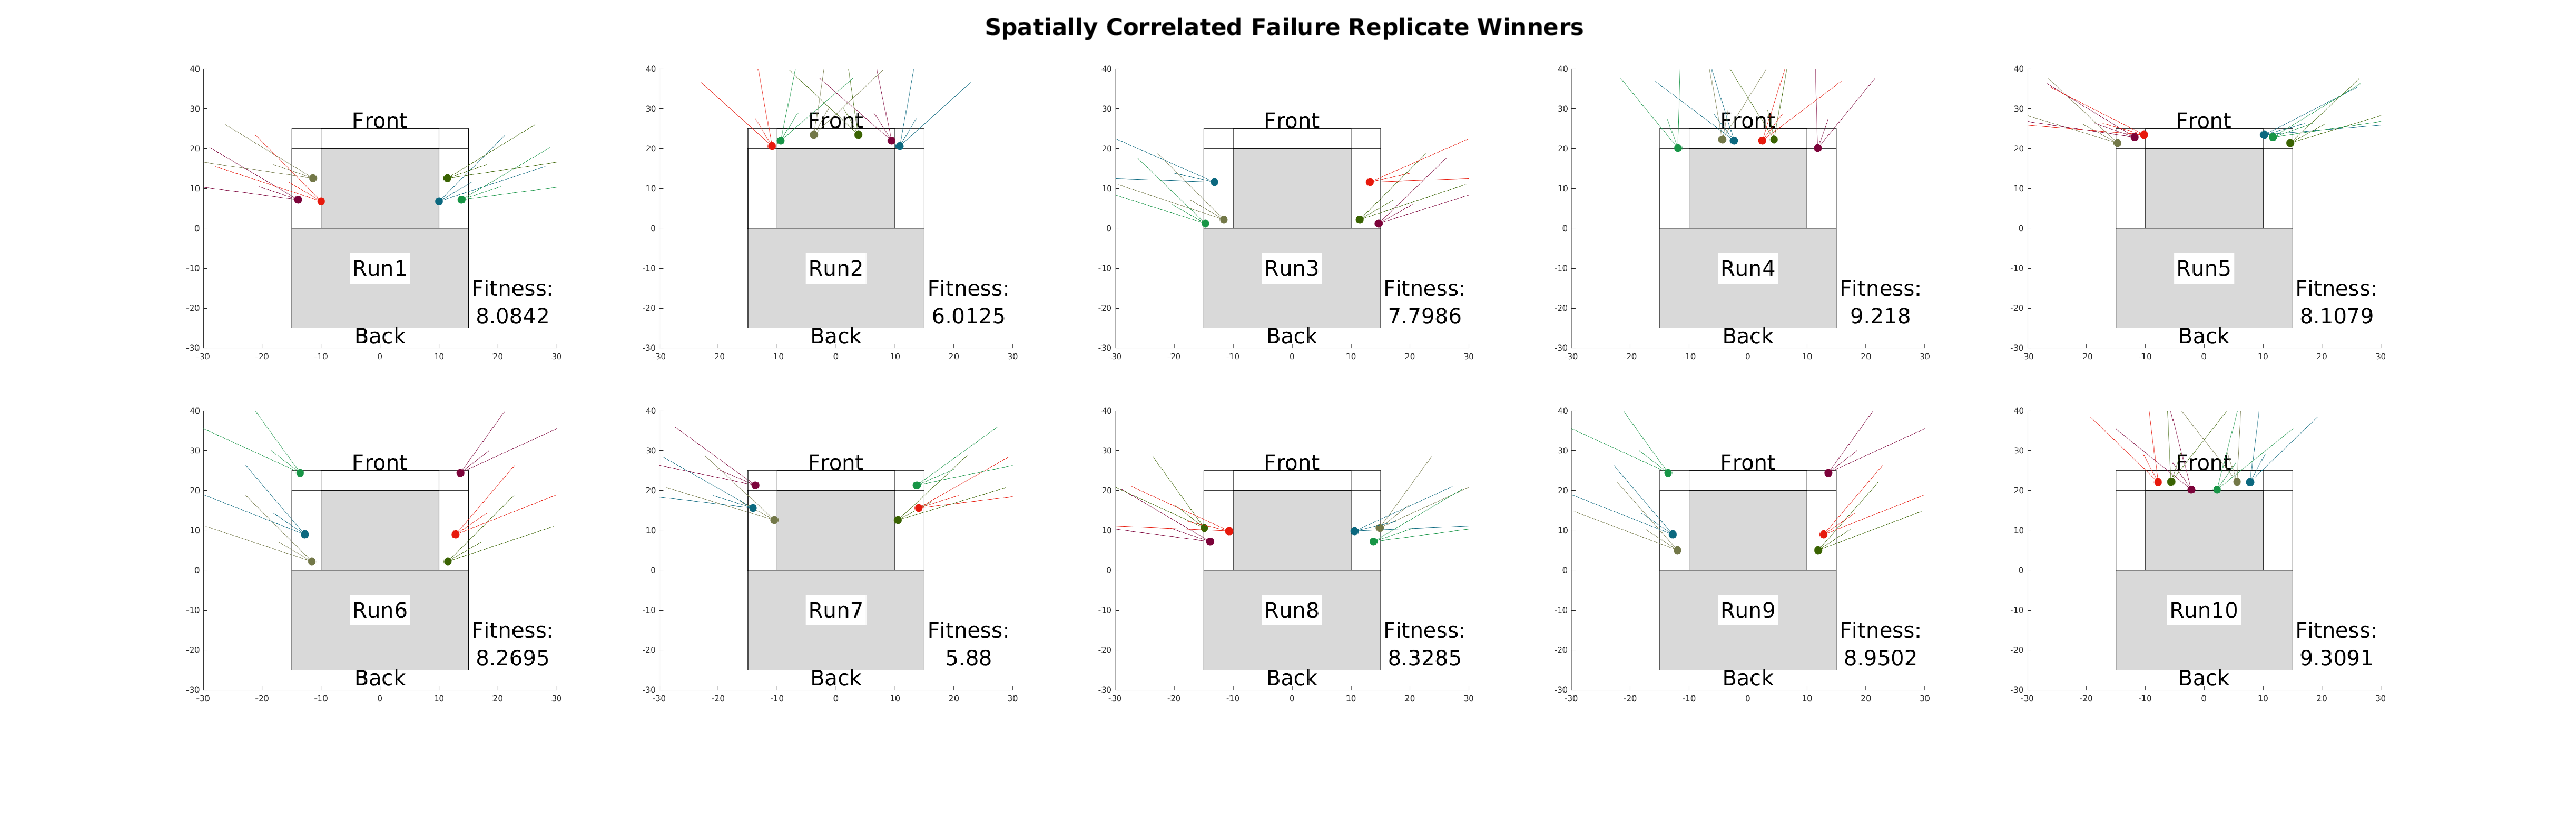
\includegraphics[width=0.95\textwidth]{Figures/6_sonar_symmetric_placement_with_aoe_failure_winners_panel_2x5.png}
    \vspace{-0.3in}
    \caption{A panel image showing winning sensor configuration for each replicate with spatially correlated failures.}
    \label{spatial_failure_panel_fig}
%    \vspace{-0.2in}
\end{figure*}




